\documentclass[letterpaper,10pt,titlepage,fleqn]{article}

%example of setting the fleqn parameter to the article class -- the below sets the offset from flush left (fl)
\setlength{\mathindent}{1cm}

\usepackage{graphicx}

\usepackage{amssymb}
\usepackage{amsmath}
\usepackage{amsthm}

\usepackage{alltt}
\usepackage{float}
\usepackage{color}

\usepackage{url}

\usepackage{balance}
\usepackage[TABBOTCAP, tight]{subfigure}
\usepackage{enumitem}

\usepackage{pstricks, pst-node}

%the following sets the geometry of the page
\usepackage{geometry}
\geometry{textheight=9in, textwidth=6.5in}

% random comment

\newcommand{\cred}[1]{{\color{red}#1}}
\newcommand{\cblue}[1]{{\color{blue}#1}}

\usepackage{hyperref}

\usepackage{textcomp}
\usepackage{listings}

\usepackage{tabularx}
\def\name{Rattanai Sawaspanich}

%% The following metadata will show up in the PDF properties

\hypersetup{
   colorlinks = true,
   urlcolor = black,
   pdfauthor = {\name},
   pdfkeywords = {ECE472 Advance Computer Architecture},
   pdftitle = {ECE472 Homework 1},
   pdfsubject = {ECE472 Homework 1},
   pdfpagemode = UseNone
}

\parindent = 0.0 in
\parskip = 0.2 in

\begin{document}

\pagestyle{empty}

\begin{center}
   \section*{ECE472 Advance Computer Architecture - Homework 3}
   Assignment 3

   Rattanai Sawaspanich
\end{center}

%\rule[0 in]{6.5 in}{0.01 in}

\section*{For a 4KB page, and a 32 bit address space, calculate the amount of memory needed to store a process's page tables. Assume each entry in the page table requires 10 bytes. Show all calculations.}
\textbf{Given: }
Each entry in Page Table has a size of 10 Bytes. 
The Page frame has the size of 4 KByte. \newline
Each entry in the Frame Page takes up 32 bits (4 bytes)\newline
\textbf{Assumption: } Each Byte conprises of 8 bits. \newline
\textbf{Solution: }\newline 
32-bit address space can be used to refer total of $ 2^{32} $ Bytes\newline
which is equipvalent to \[ \dfrac{2^{32}(byte)}{4096 (byte/page)} = 1048576 (page) \] .\newline
\textbf{Therefore, }the size of page table is $ 1048576 (page) \times 10 (byte/page) = 10485760 (byte) = 10.485 MB$

\section*{For a 4KB page, and a 64 bit address space, calculate the amount of memory needed to store a process's page tables. Assume each entry in the page table requires 10 bytes. Show all calculations.}
\textbf{Given: }
Each entry in Page Table has a size of 10 Bytes. 
The Page frame has the size of 4 KByte. \newline
Each entry in the Frame Page takes up 64 bits (8 bytes)\newline
\textbf{Assumption: } Each Byte conprises of 8 bits. \newline
\textbf{Solution: }\newline 
64-bit address space can be used to refer total of $ 2^{64} $ Bytes\newline
which is equipvalent to \[ \dfrac{2^{64}(byte)}{4096 (byte/page)} = 4.50 \times 10^{15} (page) \] .\newline
\textbf{Therefore, }the size of page table is $ 4.50 \times 10^{15} (page) \times 10 (byte/page) = 4.50 \times
10^{16} (byte) = 45 PB$

\section*{For a 8KB page, and a 32 bit address space, calculate the amount of memory needed to store a process's page tables. Assume each entry in the page table requires 10 bytes. Show all calculations.}
\textbf{Given: }
Each entry in Page Table has a size of 10 Bytes. 
The Page frame has the size of 8 KByte. \newline
Each entry in the Frame Page takes up 32 bits (4 bytes)\newline
\textbf{Assumption: } Each Byte conprises of 8 bits. \newline
\textbf{Solution: }\newline 
32-bit address space can be used to refer total of $ 2^{32} $ Bytes\newline
which is equipvalent to \[ \dfrac{2^{32}(byte)}{8192 (byte/page)} = 524288 (page) \] .\newline
\textbf{Therefore, }the size of page table is $ 524288 (page) \times 10 (byte/page) = 5242880(byte) = 5.243 MB$

\section*{For a 8KB page, and a 64 bit address space, calculate the amount of memory needed to store a process's page tables. Assume each entry in the page table requires 10 bytes. Show all calculations.}
\textbf{Given: }
Each entry in Page Table has a size of 10 Bytes. 
The Page frame has the size of 8 KByte. \newline
Each entry in the Frame Page takes up 64 bits (8 bytes)\newline
\textbf{Assumption: } Each Byte conprises of 8 bits. \newline
\textbf{Solution: }\newline 
64-bit address space can be used to refer total of $ 2^{64} $ Bytes\newline
which is equipvalent to \[ \dfrac{2^{64}(byte)}{8192 (byte/page)} = 2.25 \times 10^{15} (page) \] .\newline
\textbf{Therefore, }the size of page table is $ 2.25 \times 10^{15} (page) \times 10 (byte/page) = 2.25 \times
10^{16} (byte) = 22.5 PB$


\section*{Describe the concept of pipelining, and why it is useful.}
\textbf{Pipelining} is a method of dividing process into independent stages and move objects through stages in
sequence. At a given time, multiple objects are being processed. Fundamentally instruction pipelining is broken
up into five independent stages: Fetch, Decode, Execute, Memory-Access(Read), and Memory-Update(Write). 
Pipelining a very useful technique because it allows most (if not all) the hardware resouces to be used; it 
improves an overall system performance. Although, pipelining is a nifty techinique but there are some trade-off
. (Please take a look at next two question).

\newpage
\section*{Describe the IA-32e paging structure, in detail.}
\subsection*{Overview}
Accroding to Intel Architectures Developer's Manual, there are four levels of system data structures including 
\textbf{the Page Map Level 4, A set of page direcotry pointer tables, Sets of page directories, Sets of Page tables.}
\newline
\begin{tabular}{l p{8cm}}
   \textbf{The Page Map Level4 (PML4)} & An entry in PML4 contains a paddr of the base of a Page Directory Pointer Table. 
   The base physical address of the PML4 is stored in CR3\\
   \textbf{A set of Page Directory Pointer Table} & An entry in PDPT contains paddr point to base of Page Directory Table.\\
   \textbf{Sets of Page Directories} & An entry in Page Directory table contains the physical address of the Page Table\\
   \textbf{Sets of Page Table} & An entry in a Page Table contains the paddr of a Page (page frame). 
\end{tabular}
\newline
\newline
\textbf{NOTE: } The addressses in each data layer are 64 bits physical address value. In order for the system to be
able to keep track of all the addresses, four system-descriptor registers are required: GDTR, IDTR, LDTR, and TR.  
The registers are expanded in hardware to handle the 64 bit addressing.

Furthermore, the paging system arhitecture also follows the Operating System Instruction, Performance-monitoring counter
and Internal Caches and Buffers. The Performance-noitoring counter are event counters that counts processor event. 
Generally, a processor has multiple internal caches and buffers. The caches are used to store both data and instructions. 
The buffers are used to stored decoded addresses to the program segment and write operations waiting to be processed. 
%P.2022

\subsection*{Memory Management Registers}
GDTR, LDTR, IDTR, and TR are four system memory-management registers that contain physical addresses of the data
structures which control segmented memory mamangement. The figure below shows the format of the register layout. 
\newline
\begin{center}
   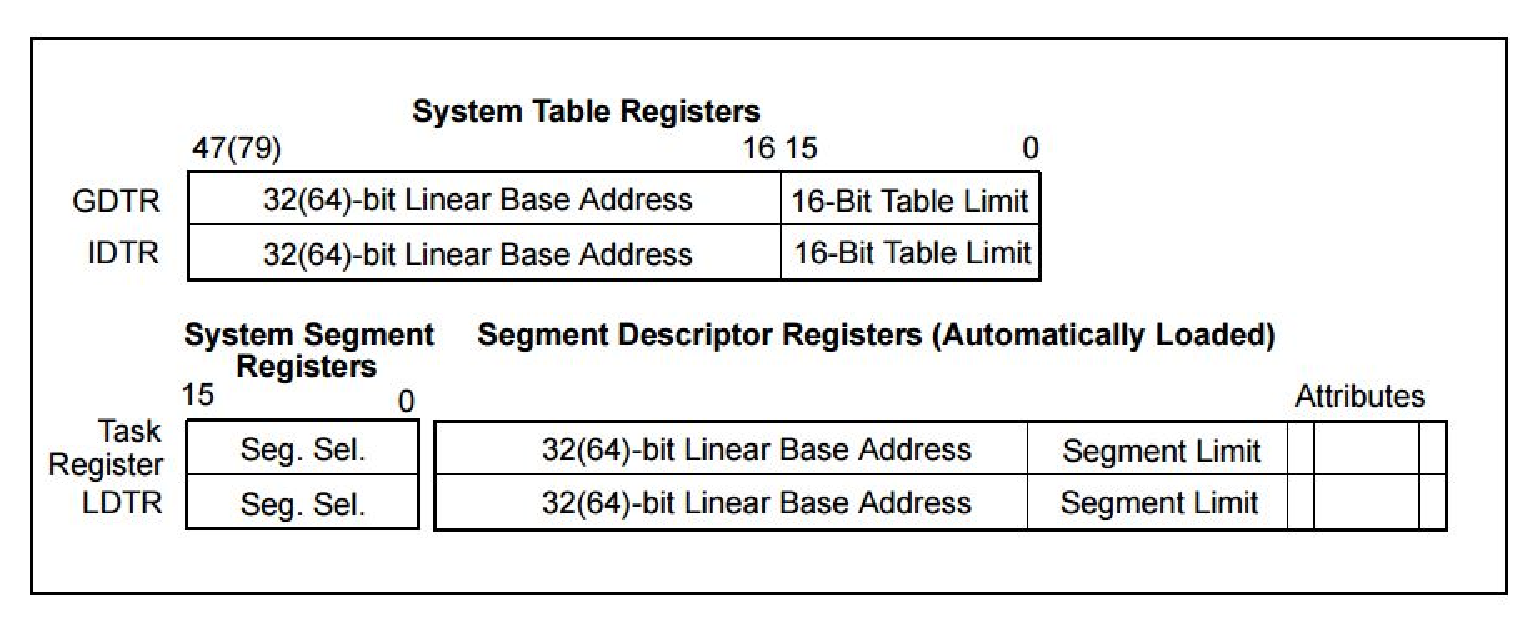
\includegraphics[width=0.8\textwidth]{system_table_reg.eps}
\end{center}
\textbf{Global Descriptor Table Rekgister (GDTR)} \newline
GDTR register contains base physical address (64 bits in IA-32e mode) and the 16-bits table limit (offset). 
The physical address points to byte 0 of GDT and the table limit (an offset) specifies the number of byte in the table. 
\newline
\newline
\textbf{Local Descriptor Table Register (LDTR)} \newline
LDTR contains the 16-bit segment selector: base address, segment limit, and descriptor attributes for the LDT. 
The base address specifies the linear address of byte 0 of LDT segment annd the segment limit specifies the number of byte 
in thesegment. 
\newline
\newline
\textbf{IDTR Interrupt Descriptor Table Register} \newline
IDTR register contains base address and 16-bit table limit for the IDT. The base address specifies the linear address of
byte 0 of the IDT and the table limit specifies the number of bytes in the table.
\newline
\newline
\textbf{Task Register (TR)} \newline
TR holds 16-bits segment selector, base address, segment limit, and descriptor attributes for the TSS of teh current task. 
The selector references the TSS descriptor in the GDT. The base address specifies the address of byte 0 of the TSS and the
segment limit specifies the number of bytes in the TSS. 
\newline
\newline
\textbf{Note: }All the register listed above are reset (set to defualt value of 0) upon power up. 
\newline
\subsection*{Paging Modes}
\begin{center}
   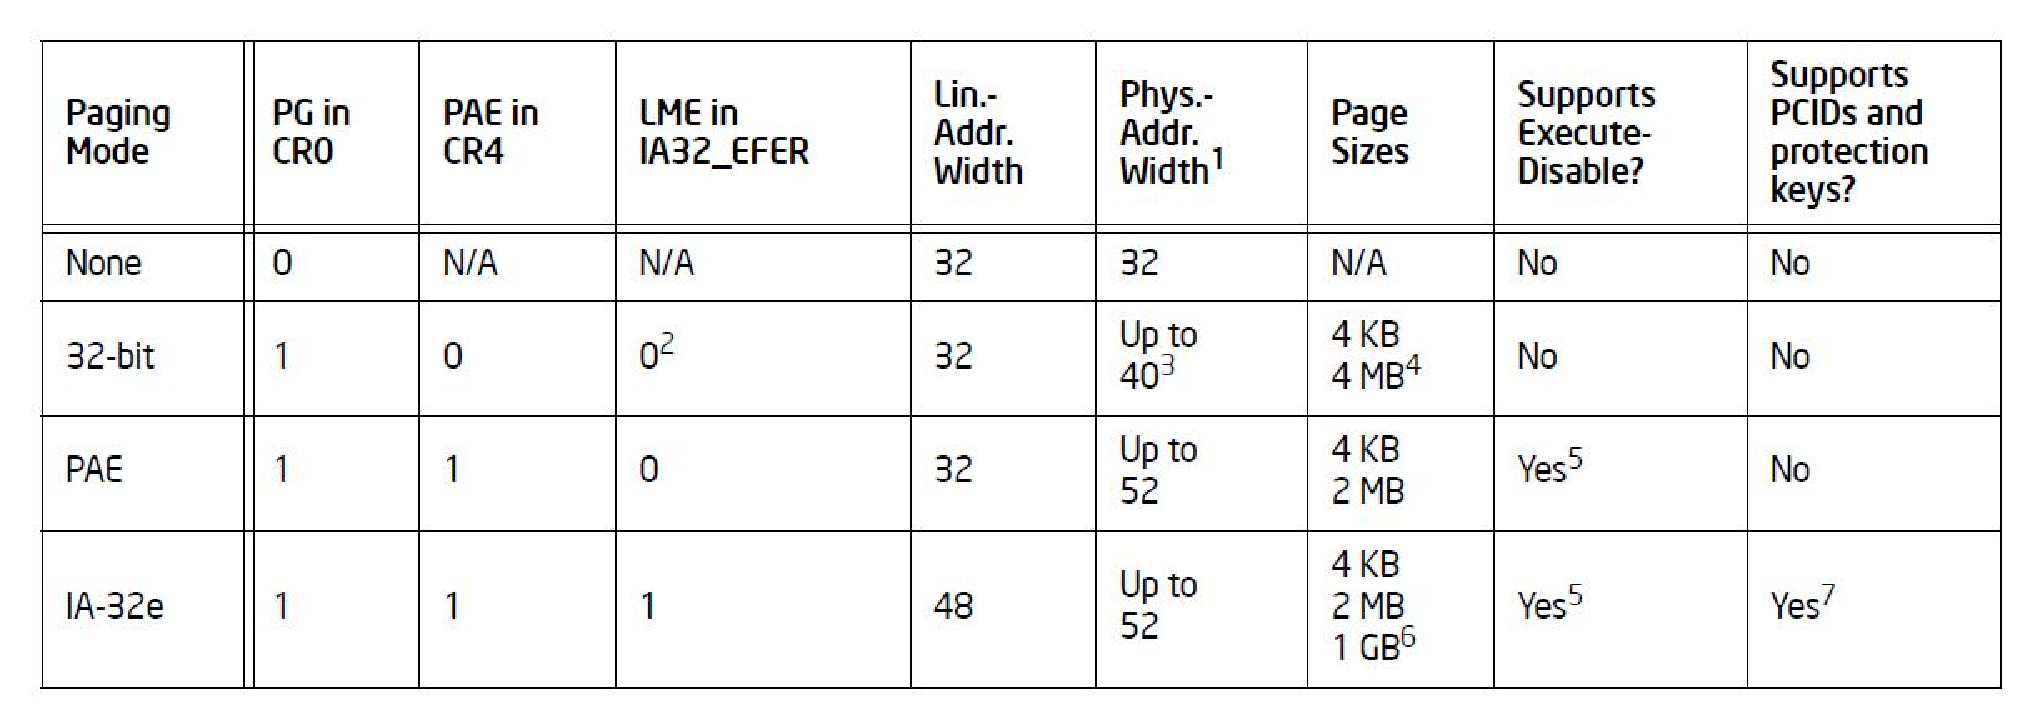
\includegraphics[width=0.8\textwidth]{paging_modes.eps}
\end{center}
\textbf{Note: }Every pageing strucuture is 4096 Bytes in size (4KB) and comprised a number of individual entires.
\newline
\newline
If CR0.PG = 0, the paging is disable and the rest of the parameters are ignored.  The logical proccessor treats all virtual address as if they were physical physical addresses. 
\newline
\newline
If CR0.PG = 1, the paging is enable if the protection is also enable (CR0.PE = 1). 
There are three modes of paging: 32-bit paging, PAE paging, and IA-32e paging. \newline
\newline
\textbf{32-bit paging} [CR0.PG = 1 and CR4.PAE = 0] \newline
In the 32-bit paging mode, each entry is 32 bits (4 bytes); there are 1024 entires in each strucutre. 
\newline
\newline
\textbf{PAE paging}    [CR4.PAE = 1 and IA32-EFER.LME = 0] \newline
In PAE paging mode, normally each entry is 64 bits (8 bytes); there are 512 entires in each structure.
Except when the mode is specified to have each entry size of 32 bytes; there are \textbf{four} 64-bit entries.
\newline
\newline
\textbf{IA-32e paging} [CR0.PG = 1, CR4.PAE = 1, and IA32-EFER.LME = 0] \newline
In IA-32e paging mode, each entry is 64 bits (8 bytes); there are 512 entires in each structure.
\newline
\newline
\textbf{Note: } For a specific configuration i.e. page size, supervisor mode, execution rights. Pleaes take a
look at \textbf{Paging-Mode Modifiers} in Intel 64 and IA-32 Architectures Software Developer's Manual Vol.3 
section 4.1.3.

\subsection*{Paging Translation}
The processor uses the higher portion of a logical address to identify a series of paging-structure entires.
The last of these entries contains the physical address of the region to which the virtual address translates.
(a Page Frame). The lower portion of the logical address is a Page Offset that specifies the address within 
the page frame.
Each paging-structure contains a physical address that either the address of another paging structure (referencing) or the address of a Page Frame (mapping a page).
\newline
\begin{center}
   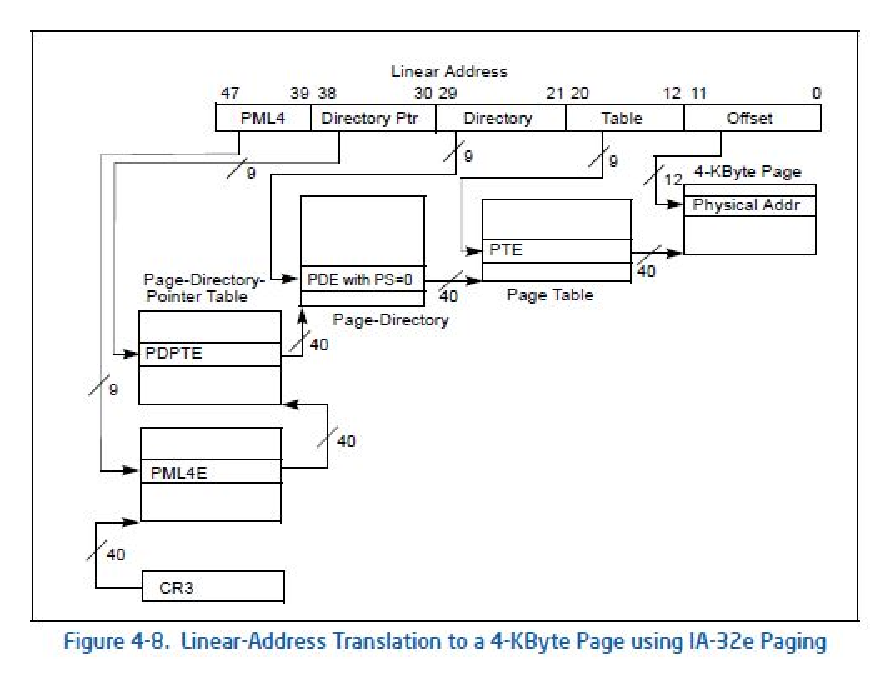
\includegraphics[width=0.8\textwidth]{trans_IA32e_4KB.eps}
\end{center}
For an example in case of IA-32e Paging mode, the processor starts at CR3 register looking into bit M-1:12 for
a physical address of the 4KB aligned PML4 table.  Then the processor would resolve to PML4 entry, look into 
bit M-1:12 for address of the page-directory-pointer table (PDPTE). In PDPTE, the processor looks for the 
address of page director (PDE), bit M-1:12, and the PDE offset, bit M-1:30. Afterwards, the processor resolves
to the PDE and select a byte with the PDE offset to obtain an address to 2MB-page frame and address of page 
table (offset). In 2MB-page frame, the processor would look for the address of 4KB page frame and the offset
from the original logical address to resolve for the translated physical address. 

\textbf{Note: } For more detail of the bit layout, please take a look at P.2084 of Intel SDM Vol.3 
%P.2062
\newpage

\section*{What are some examples of pipeline hazards, and what are some ways of dealing with them?}
\subsection*{Complexity}
\begin{itemize}
   \item The more pipelining stages, the more prone there is to the system errors. It is because of the 
      complexity of how the instructions are breaking up and how to the data path layout. For a piplining 
      to be resilient, the system requires to have a better error handler.  
   \item The edge cases can be very tricky in a pipelining architecture. There are multiple blocks
      of instructions and each of them have their own unique edge-cases that may cause a system failure or
      an unpredictable result.
\end{itemize}

\subsection*{Non-Determinism}
\begin{itemize}
   \item You cannot guarantee the actual execution time for each instruction because the run time of the 
      current instruction also depending on the empty stages there are from the previous instructions.
      Although, you can still find an accurate average run time for an instruction.
   \item Pipelining cannot really be used in a system that requires a synchronization in a high 
      clock frequency. It is due to the propagatoin delay at the hardware level; an electron moving 
      through a wire takes time. 
   \item Branching in a pipelining is a nightmare because if the destination stage is currently in used,
      the stage will be flushed in replace with the instruction. Thus, the system takes a severe 
      performance panalty.
\end{itemize}

\subsection*{Instruction Ordering}
\begin{itemize}
   \item Intel has an out-of-order instruction execution. With pipelining the complexity of the system just
      goes off the roof.  Moreover, the order of the execution (even though it is out of order) needs to be
      re-arrange to optimize the performance of the pipeline. 
   \item Typically, a program would have to Read/Write a section of data. In pipelining, it is possible for a
      program to accidentally get a piece of an outdated data becaues a piece of data is being processed on
      a different stage in the pipeline. 
\end{itemize}


\end{document}

